\chapter{Présentation du système}
\label{presentation_systeme}
\lhead{Chapitre 3 - Présentation du système}
\section{Introduction}

Ce chapitre vise, à l'aide d'un exemple concret d'utilisation,  à:
\begin{enumerate}
\item introduire les technologies utilisées pour développer l'application;
\item expliquer les différentes fonctionnalités de l'application d'un point de vue utilisateur. Les utilisateurs étant de deux types, la section relative aux fonctionnalités sera divisées en deux parties. Dans un premier temps, nous expliqueront les fonctionnalités offertes à la commission de programme à savoir;
  \begin{itemize}
    \item l'import de données dans l'application (Programmes de cours, modules, cours);
    \item la gestion des données (Accéder au différents cours, modules et programmes, mettre à jour leur données);
    \item la gestion des contraintes;
    \item comment vérifier les programmes de cours des étudiants.
  \end{itemize}
Ensuite, nous présenterons ce qu'il est possible de faire en tant qu'étudiant avec l'application à savoir:
\begin{itemize}
  \item se créer un compte utilisateur;
  \item se connecter avec son compte utilisateur;
  \item se créer (ou modifier) un programme de cours, en choisissant le programme à suivre;
  \item configurer son programme de cours, en configurant les différentes années qui le compose et en choisissant les modules de cours à suivre;
  \item vérifier la validité de son programme;
  \item négocier avec la commission de programme la justification des exceptions. 
\end{itemize}
 
\end{enumerate}

Un des principaux objectifs de ce mémoire étant d'offrir une solution maintenable et évolutive, l'application est divisée en trois parties distinctes, indépendantes entre elles. 

Ces trois parties sont les suivantes:
\begin{itemize}
\item l'import et la mise à jour des catalogues, de ses programmes, modules, cours et des différentes contraintes par la \textit{commission de programme}; 
\item la création du programme par l'étudiant, via l'interface utilisateur;
\item la vérification (par l'application) des différentes contraintes induites par le programme créé précédemment par l'étudiant.
\end{itemize}

\subsection{Exemple d'utilisation}

Tout au long de ce chapitre, l'exemple suivant va être utilisé pour illustrer le fonctionnement de l'application. Il s'agit d'un catalogue de cours fictif proposant deux programmes de cours. Ce programme fictif se rapproche très fort de la réalité. Certaines parties du catalogue (Certains modules optionnels du programme de master, certains cours) on été élaguée pour rendre l'exemple plus clair. L'exemple n'en reste pas néanmoins représentatif de la réalité, il comporte en effet les différents types de contraintes que l'on peut rencontrer par exemple. 
\begin{figure}
\centering
\caption{Exemple fictif de catalogue de cours}
\label{fig:running_example}
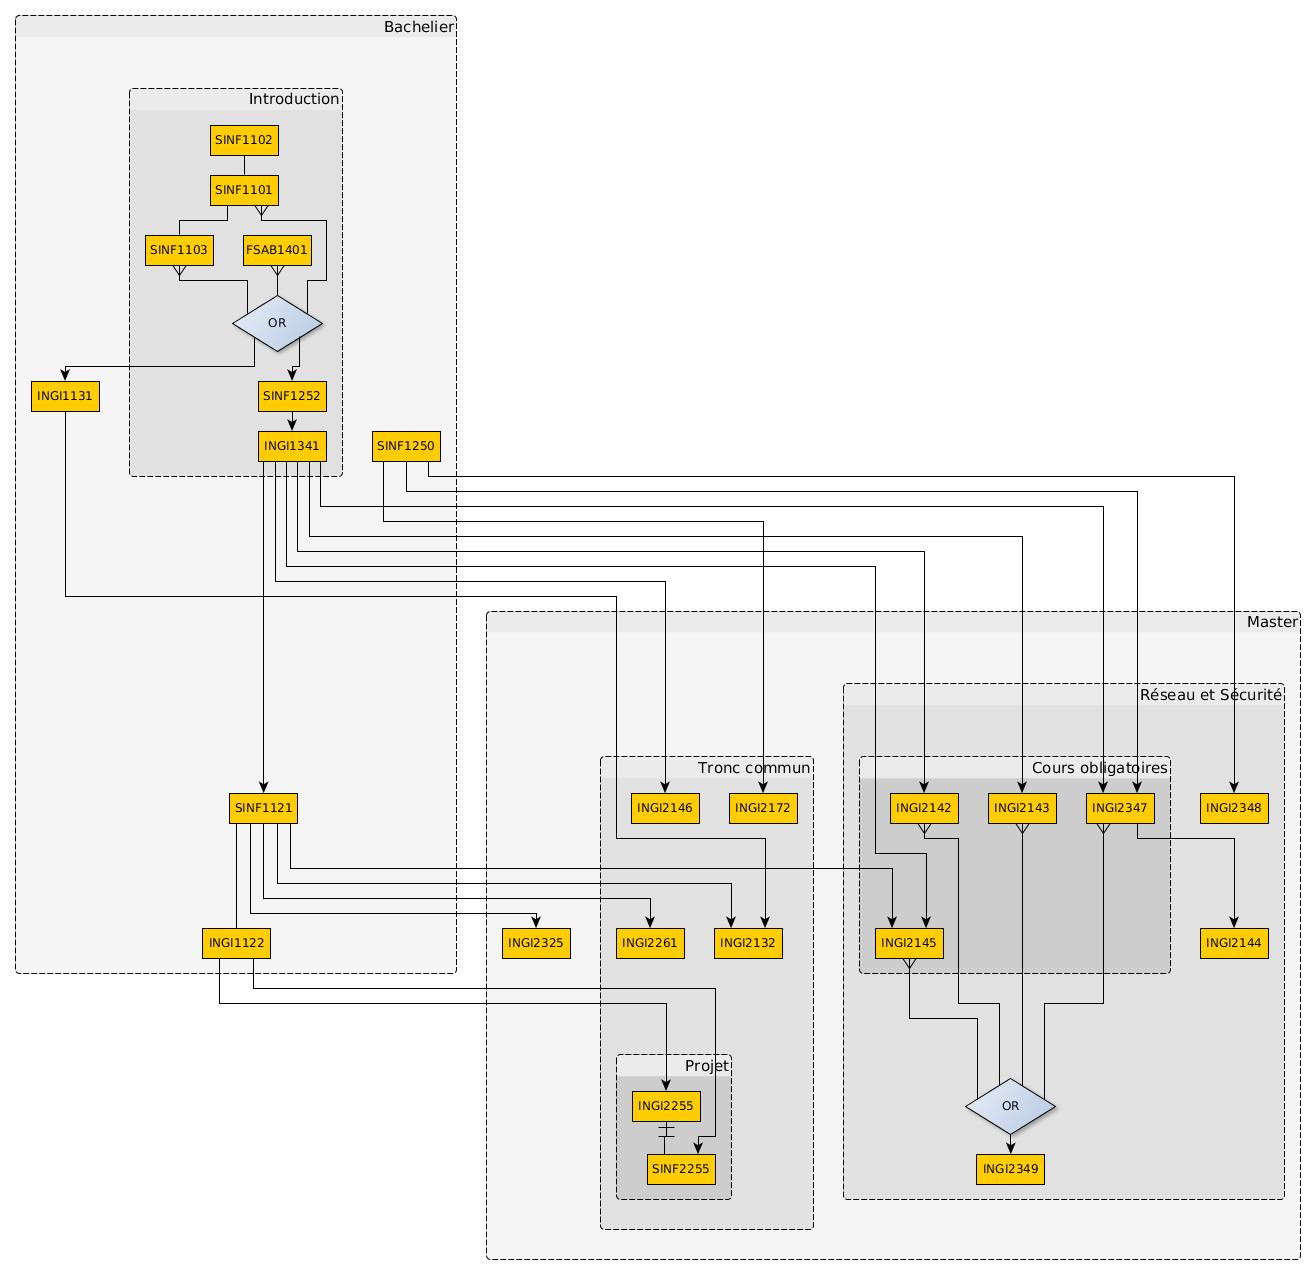
\includegraphics[width=\textwidth]{running_example}
\end{figure}

Ce catalogue est composé de deux programmes de cours.

Un programme de \textbf{Bachelier} (le grand rectangle à droite de la figure \ref{fig:running_example}) composé d'un module obligatoire (Introduction, la petite boite imbriquée s’appelant \textit{Intro})

Un programme de \textbf{Master} (le grand rectangle à gauche de la figure \ref{fig:running_example}) composé d'un module optionnel (L'option réseaux et sécurité, la boite imbriquée à gauche) et d'un module obligatoire (Le tronc commun, la boite imbriquée à droite). De plus, certains cours de master dépendent de cours de bac. 


%************************************************************
\section{Technologies utilisées}
\subsection{Introduction}
Le but poursuivit par cette section est de présenter les différents choix faits aux niveaux des technologies utilisées par l'application. Ces choix sont de deux types. Premièrement, les technologies utilisées pour construire l'application seront présentées, comme le framework ou la base de données qui est utilisée. Les technologies externes à l'application qui sont utilisées pour construire les différents curricula ou mettre à jour leur informations seront présentées par la suite.

On parle de technologie interne pour représenter celles qui sont utilisées pour développer les fonctionnalités de application. Les technologies externes sont quant à elles des applications déjà existantes qu'il faut utiliser \textbf{en dehors} de l'application et pour lesquelles il ne faut pas écrire de lignes de codes.
\subsection{Ruby on Rails}
\subsubsection{Introduction}

Cette section a pour but de présenter la technologie principale utilisée pour développer l'application. Le but n'est pas de parcourir en détails le fonctionnement de Rails, mais bien d'en présenter les concepts clés. En effet, il semble important d'en comprendre les grande lignes, car son architecture, aussi bien que ses principes ont influencé la structure de la solution.
\subsubsection{Le choix d'un framework}
A première vue, l'utilisation d'un framework n'est pas absolument nécessaire. Cependant, un framework apporte toute une collection d'outils qui aident à développer mieux et plus rapidement.

\textbf{Mieux} car il permet de développer une application qui est structurée, ce qui rend le code plus maintenable et évolutif.

\textbf{Plus rapide} car il permet de gagner du temps en réutilisant des modules génériques afin de se concentrer sur d'autres domaines. Avec un framework, on assemble des briques plutôt que de réinventer la roue. 

Enfin, le dernier atout d'un framework se situe au niveau de l'intégration de nouveaux développeurs sur le projet. Dans le cadre de ce mémoire, il est clair que de nouvelles fonctionnalités devront être ajoutées dans le futur. De plus, les fonctionnalités existantes devront peut être modifiées ou améliorées. Il sera plus facile pour cette personne de se plonger dans du code qui n'est pas le sien, s'il a une structure propre aux standard web d'aujourd'hui.

\textbf{Il est donc fortement conseillé d'utiliser un framework web pour créer ce genre d'application.} 

Il en existe une multitude aujourd'hui. Il y a tout d'abord les frameworks PHP comme CakePHP, DRUPAL ou Symfony (pour ne citer que les plus connus). Vient ensuite Ruby on Rails, un framework en ruby et Django, un framework en Python. Cette liste n'est bien entendu pas exhaustive. 
\subsubsection{Le choix de Ruby on Rails}
L'intérêt réside dans le niveau de productivité et de maintenabilité accru que l'on obtient en travaillant avec le framework. Les design patterns sous-jacents, et la philosophie de Rails permettent de concentrer son travail sur les fonctionnalités de l'application plutôt que de passer son temps à écrire du code répétitif ou remplir des fichiers de configuration. 

De plus, il existe une multitude de librairies tierces appelées \textit{ruby-gem} qui réduisent encore le nombre de lignes de codes à produire, en apportant des fonctionnalités à l'application. Le meilleur exemple est \textbf{devise}, une librairie qui permet d'ajouter la gestion de l'utilisateur(création, connexion, récupération de mot de passe, envois de mails, etc ..) en quelques lignes en plus de gérer les sessions et les accès aux différentes actions et vues. 

Rails pousse aux bonnes pratiques, c'est d'ailleurs cette philosophie qui m'a incité à développer la plupart des fonctionnalités, comme vous le verrez plus tard, dans des librairies externes à l'application.


En outre, Rails dispose d'une communauté très active et passionnée, qui teste, documente et améliore les fonctionnalités du framework. 

Les limites du framework sont les suivantes
\begin{itemize}
\item Lorsque l'on débute, on est souvent tenté de charger les modèles en voulant suivre la philosophie \textit{tiny view - skinny controller - fat model}\footnote{Bonne pratique qui consiste à délaisser toute la logique aux modèles} et l'on oublie souvent qu'il est possible de déléguer la plupart des fonctionnalités à des librairies externes, qui sont plus faciles à développer - car crées en pure \textit{ruby} - et plus facile à tester - car indépendantes de rails \cite{fat_models}.

\item Un des principaux aprioris sur les frameworks et particulièrement Ruby on Rails, est qu'il sont lents (et peu efficace). En effet, ruby est un langage interprété . Ce type de langage tend à être plus lent que les langages compilés. Cependant, il faut garder à l'esprit qu'écrire du code, trouver et corriger des bugs ou encore ajouter des nouvelles fonctionnalités dans une application sont des tâches encore plus couteuses en temps. Rails permet de réduire le temps consacré à ces tâches, ce qui est bien plus important lorsque l'on développe ou maintient une application, particulièrement dans le cadre d'un mémoire. Ainsi, à la place de configurer le mapping entre ces différentes ressources, on utilise un convention.
\end{itemize}

\subsubsection{Conclusion}
Le choix s'est naturellement porté vers Ruby on Rails. C'est un framework open-source, utilisé pour développer des applications web. Le développement se fait à travers le langage de programmation multi-paradigmes (Programmation fonctionnelle, orientée object, ...) \textbf{ruby}. Il se base sur des puissants design patterns et principes qui vont être présentés en quelques lignes ci-dessous.

\subsubsection{DRY - Don't repeat yourself}
Comme son nom l'indique, ce premier principe pousse à la réutilisation du code existant le plus souvent que possible, plutôt que d'avoir des bout de codes similaire un peu partout dans l'application. L'idée de tendre vers une structure \textit{Api}, où tout ce qui n'est pas nécessaire aux classes et méthodes externes est caché en interne. Le principal avantage se situe au niveau de la \textbf{maintenabilité}. On évite ainsi de devoir partir à la recherche des différents bouts de code dupliqués lorsque l'on veut modifier le comportement d'une méthode, d'une classe, ou même d'un module.

\subsubsection{CoC - Convention over Configuration}
L'idée est de réduire au minimum les décisions à prendre avant de commencer à développer. Une convention importante en \textit{Ruby on rails} se situe au niveau des noms des classes pour lesquelles il existe une table correspondante en base de données. Pour un modèle \textit{Course} par exemple, la convention est d'avoir une table nommée \textit{courses} en base de données. Cela permet d'éviter d'avoir à écrire du code supplémentaire pour spécifier à l'application quelle table correspond à quel objet. 

Cela permet au développeur de se concentrer sur les parties non conventionnelles de l'application, comme l'architecture, plutôt que de perdre son temps à configurer les objets. L'avantage ici se situe plus au niveau de la \textbf{productivité}.
\subsubsection{MVC - Model-Vue-Controlleur}

Le framework s'appuie sur le pattern \textbf{MVC}. Destiné aux applications dites \textit{interactives}, il divise l'application en trois parties; le modèle, les vues et le contrôleur. Notez que \textit{Ruby on Rails} ne respecte pas totalement MVC dans sa conception initiale. Cela se justifie par le fait que ce pattern n'est pas destiné à la base aux applications web, notamment car la vue est ici une page web. Le modèle ne peut donc pas lui envoyer tous les changements qui surviennent au niveau des données. C'est la vue, qui doit expressément faire les requêtes pour ces données, à travers le contrôleur.

MVC à la sauce Rails se présente comme suit. Nous avons:

\begin{description}
\item[le modèle] lié à une base de données, qui contient les données et l'état de l'application. Il contient aussi tout les objets métiers \footnote{Objets qui font tout le travail.}, qui détermine comment l'information est créée, mise à jour, et affichée;
\item[les vues] qui génèrent l'interface utilisateur et lui présentent les données. Ce composant est passif, il ne traite aucune information. \textit{Vues} est au pluriel ici, car plusieurs vues peuvent avoir accès au même modèle;
\item[le contrôleur] qui reçoit les événements du monde extérieur, interagit avec le modèle et choisit la vue à afficher à l'utilisateur. Par exemple, lorsque l'utilisateur veut éditer un commentaire dans un blog, le contrôleur va rendre la vue relative à l'édition de l'objet correspondant. 
\end{description} 

\subsubsection{Active Record}
Ce pattern quant à lui stocke les données dans une base de données relationnelle. Il s'agit simplement de fournir une abstraction supplémentaire à la base de données et fournir des fonctions pour manipuler les données. Dans le cas de rails, il y a donc une couche ruby entre la base de données proprement dite et la logique dans notre modèle. Cela permet par exemple, d'être indépendant du système de base de données utilisée en dessous.  Par exemple, \textit{postgresql} est le système de gestion de base de données utilisé pour le moment (source : \cite{rails_cast_migration_to_postgresql}. Si pour une raison X ou Y, il devient nécessaire de passer à \textit{sqlite3}, il suffit de changer le fichier de configuration \textit{config/database.yml} de
\begin{lstlisting}
development:
  adapter: postgresql
  database: db/development
  pool: 5
  timeout: 5000
\end{lstlisting}
vers
\begin{lstlisting}
development:
  adapter: sqlite3
  database: db/development
  pool: 5
  timeout: 5000
\end{lstlisting}

Et de recréer la base de données avec
\begin{lstlisting}
rake db:create:all
rake db:migrate
\end{lstlisting}



Tout cela est fait sans devoir changer comment sont accédées les données dans les différents modèles.  

\subsection{Base de données - PostgreSQL}

Rails supporte plusieurs systèmes de gestion de base de données : PostgreSQL, MySQL, SQLite. Le choix du système est cependant restreint à la plateforme utilisée pour héberger l'application (Heroku). En effet, il est nécessaire d'avoir une base de données PostgreSQL pour pouvoir héberger l'application sur Heroku. 

\subsection{Éditeur de graphes - yEd}
\label{yed}
Comme expliqué plus tard dans la section \ref{data_mgmt} détaillant comment sont importés les données, le choix s'est porté vers une importation en deux étapes des données dans l'application. 

\textbf{La première étape} consiste à créer et importer le graphe de cours. Les données importées durant cette étapes sont les nom identifiant les différents objets du graphes (cours, programme, podule), la structure des différents programmes de cours (les cours et modules constituant les programmes de cours) et les dépendances entre les cours.\footnote{Se référer à la section \ref{dependances} (relative aux dépendances) pour plus de détails.}

\textbf{La deuxième étape} consiste à ajouter des nouvelles données des différents objets (ou les mettre à jour) à l'aide d'un formulaire excel. Cela permet d'ajouter des propriétés comme les crédits d'un cours ou les crédits minimum requis d'un programme de cours par exemple.\footnote{Se référer à la section \ref{properties} pour plus de détails.} 

Le but de cette section est d'expliquer les choix qui on été faits aux niveau des technologies utilisées pour s'occuper de \textbf{la première étape} (La construction d'un graphe). 

Pour construire et importer le graphe de cours, plusieurs alternatives se sont présentées.

La première correspond à un logiciel intégré dans l'application, qui permet de construire explicitement un catalogue de cours sous forme de graphe, en proposant exclusivement de placer des objets cours, modules, ou programmes sur le graphe et en n'offrant que des arrêtes de type corequis ou prérequis. Cette application communiquerait directement avec les modèles et permettrait de générer directement les objets (cours, modules, ...) désirés. Cependant il n'existe pas d'applications réalisant ce genre de graphe pour le moment. Il faudrait donc développer un outil, intégré dans l'application,  fournissant ces fonctionnalité. Cependant, cela sort du cadre de ce mémoire, faute de temps. 

La deuxième alternative serait d'intégrer un outil générant des graphes plus standard dans l'application. YWorks offre une solution, yFiles, qui est permet la création et l'édition de graphes en HTML5 et en javascript. Ce logiciel est cependant très chère.

La troisième et dernière alternative serait d'utiliser un logiciel externe à l'application pour générer ces graphes. Ce logiciel, en plus d'être gratuit, doit être multi-plateformes (Mac os x, Linux \& Windows) et capable d'exporter dans un format relativement facile à parser. La liste de ce genre de logiciel est assez longue (Dia, Yed, OmniGraffle, Graphiz)
\begin{itemize}
  \item Dia - C'est un logiciel assez léger qui est capable d'exporter en Xml, un format standard pour représenter des données. Il devient cependant très ennuyeux à utiliser lorsque l'on manipule des graphes de taille importante. C'est cependant un éditeur graphique très générique qui n'est pas seulement destiner à la création de graphes. 
  \item OmniGraffle - Ce logiciel n'est disponible que sur Mac Os X malheureusement.
  \item Yed - Ce logiciel est assez complet. Il est cross-plateforme et à l'avantage de contenir des algorithmes qui permettent de restructurer automatiquement les graphes. Il permet aussi d'exporter en deux formats de types xml (Graphml \& XGml)
  \item (...)
\end{itemize}

Étant donné la contrainte de temps imposé par le cadre du mémoire, le choix s'est porté vers un logiciel déjà existant. Il a été préférable de choisir une solution externe pour éviter de surcharger l'application avec de lourds modules graphiques. De plus, intégrer ce genre de logiciels dans l'application ne changeait rien au fait qu'il fallait parser le fichier exporté par l'outil pour importer les données dans l'application.

YEd a été choisi pour toutes ces raisons. 
\clearpage
%*********************************************************************************************************************************$
\section{Conception}
\subsection{Introduction}
 
L'application est la  plateforme qui tient le rôle d'intermédiaire entre la commission et les étudiants. Elle est représentée par l'entité \textit{Application} sur le diagramme \ref{fig:desired_process}. Il y a trois modules attachés à cette entité.

\textbf{Le module d'import de données} - Il permet à la commission d'enregistrer les données liées aux curricula  à l'aide de plusieurs supports (qui seront expliqués en détail plus loin dans le chapitre). Ce module permet tout d'abord d'ajouter considérablement plus d'informations dans le support confié à l'étudiant pour qu'il construise sont programme. Ensuite, il permet à la commission de mettre à jour facilement ces informations. 
 
\textbf{Le module de gestion des contraintes} - Il vérifie la validité des programmes créés par les étudiants.L'intérêt de ce module est de réduire considérablement  le temps que doit consacrer la commission à la correction des programmes d'étudiants. Premièrement, il empêche les étudiants d'envoyer leur programme à la validation s'il n'est pas correcte. il fourni aux étudiants un compte-rendu en temps réel de l'état de leurs programmes, en leur pointant les parties qui ne respectent pas les contraintes, quelles contraintes ne sont pas respectées et ce qu'il faut changer dans leur programme pour y remédier.

\textbf{La base données} - Elle stocke les informations liés aux curricula enregistrés précédemment par la commission, mais aussi les programmes des étudiants. La commission pourra avoir accès aux anciens programmes de cours et à toutes les programmes des étudiants. Ces derniers quant à eux, pourront accéder aux différents programmes qu'ils ont déjà suivit et avoir une vision claire de ce qu'il leur reste à valider pour voir leur diplôme.

Les fonctionnalités de l'application, telles qu'elles apparaissent sur la figure \ref{fig:desired_process} vont être expliquées dans les sous-sections qui suivent.
\subsection{Gestion des données}
\label{data_mgmt}
 
\subsection{Contraintes}
\label{contraintes}
Comme présenté dans le chapitre \ref{contraintes_intro} précédent, les contraintes sont de plusieurs types. Le but de cette section n'est pas de recommencer leur énumération mais plutôt de présenter les choix que cette catégorisation impose de faire et d'expliquer plus en détails la logique intrinsèque des plus compliquées d'entre elles.    

Comme expliqué dans les sections qui suivent, la location des informations relatives aux contraintes (les crédits et les dépendances d'un cours par exemple) n'est pas la même pour toute les contraintes. Qui plus est, chaque contrainte n'est pas vérifiée de la même façon. Une dépendance par exemple implique d'aller chercher si un cours est présent dans un programme, alors que le minimum de crédits requis d'un programme implique de compter les crédits de chacun ces cours. Dès lors, pour ne pas surcharger les modèles de l'application et la rendre plus flexible, la vérification de ces contraintes a été déléguée à un module externe. On évite, ainsi, de se retrouver avec des modèles dont la taille se chiffre en milliers de lignes de code. 
\subsubsection{Dépendances}
\label{dependances}
Comme expliqué précédemment les dépendances peuvent être des prérequis ou des corequis. En plus de cela, ces contraintes peuvent être:
\begin{description}
\item[binaire] car elle concerne deux cours; un cours \textit{source} et un cours \textit{destination}; le sens de la contrainte étant celui de la flèche (le cours source est le prérequis du cours destination par exemple);
\item[n-aire] car elles sont composées de plusieurs cours \textit{sources} et de plusieurs cours \textit{destinations}.
\end{description}

Conceptuellement, un ensemble n-aire est un ensemble de contraintes binaires. En effet, cela revient à créer pour chaque cours \textit{destinations} une contrainte binaire pour chacun des cours \textit{sources}. 

De plus, une condition s'applique sur chacun des ensembles n-aires de dépendances. Cette condition est soit une disjonction (OR), soit une disjonction exclusive (XOR). L'effet de la condition est la suivante;

\begin{itemize}
\item Pour un ensemble disjonctif, la contrainte ne sera valide que s'il existe au moins une des sous-contraintes qui est vraie;
\item Pour un ensemble disjonctif exclusif, la contrainte ne sera valide que s'il n'existe qu'une et une seule des sous-contraintes qui est vraie.
\end{itemize}

Il y a un exemple de chaque qui se trouve dans l'exemple fictif \ref{fig:running_example}. L'ensemble disjonctif se trouve dans le programme de Bachelier. L'ensemble disjonctif exclusif quant à lui se trouve dans l'option Réseau et Sécurité du programme de Master.

\begin{figure}
\centering
\caption{Contrainte n-aire disjonctive}
\label{fig:nary_constraint}
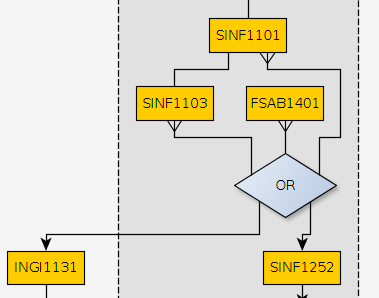
\includegraphics[width=\textwidth]{nary_constraint}
\end{figure}


Sur l'image \ref{fig:nary_constraint} apparait en détail l'ensemble disjonctif;
\begin{itemize}
  \item \textit{SINF1252} et \textit{INGI1131} sont les cours \textit{destinations}
  \item \textit{SINF1101} \textit{SINF1103} et \textit{FSAB1401} sont les cours \textit{sources}
\end{itemize}

Ces contraintes étant des prérequis, il est donc nécessaire d'avoir suivit et réussi \textit{SINF1103} \textbf{OU} \textit{SINF1101} \textbf{OU} \textit{FSAB1401} pour pouvoir suivre \textit{SINF1252} \textbf{OU} \textit{INGI1131}

Notez que les dépendances sont importées à l'aide du logiciel yEd \ref{yed}. Il n'est donc pas possible de les modifier une fois le graph importé dans l'application. 
\subsubsection{Contraintes s’exerçant sur les propriétés des cours, modules et programmes}
\label{properties}
Ces contraintes regroupent plusieurs catégories de contraintes au sens où elles on été présentée dans le chapitre \ref{contraintes_intro}. On dit que ces contraintes portent sur des propriétés car leur validité dépend de l'information contenues dans celles-ci. Pour reprendre l'exemple du minimum de crédits requis pour valider un programme de cours. La validité de cette contrainte dépends (en plus des cours et modules qui compose ce programme) de deux choses:
\begin{enumerate}
  \item la valeur de cette propriété MIN, contenue dans la propriété du même nom de l'objet Programme;
  \item la valeur de la propriété CREDITS qui compose chacun de ses cours
\end{enumerate}

Il est évidemment nécessaire que cette contrainte soit vérifier par le module qui les vérifie. Pour une contrainte temporelle comme le semestre durant lequel est dispensé un cours par exemple, la validité dépend aussi de la propriété de l'objet en question (SEMESTER)

Par contre, le module de contraintes n'a pas besoin de vérifier cette contrainte, car la configuration de chaque année se fait par semestre. Il n'est donc pas permis aux étudiants de choisir un cours, pour un semestre donné, qui n'est pas dispensé pendant ce semestre. 

Les données relatives à ces propriétés sont importées et mise à jour par le module qui s'occupe d'importer les formulaires excels. Elle peuvent donc être, contrairement aux dépendances, modifiées quand on le souhaite.  
\subsection{Fonctionnalités de l'application - Commission de programme}
\subsubsection{Introduction}
 Une fois connecté à l'aide du compte admin, nous arrivons à la page illustrée sur la figure suivante \ref{fig:landing_page_admin}. Quatre menus sont accessible depuis la barre de navigation (en haut dans la page d’accueil):
 \begin{description}
  \item [Catalogue] Ce menu offre l'accès à la gestion des catalogue. C'est ici que les catalogues sont importés (via le graph yEd) et mis à jour (via le formulaire excel). Ce menu permet aussi de gérer les versions des catalogues, pour permettre de mentionner quel est le catalogue principal (celui qui sera utilisé par défaut par les étudiants), quels sont les anciens catalogues (Pour permettre aux étudiants d'avoir accès aux anciens programmes de coues) et quel sont les futurs catalogues qui, toujours en construction, ne sont pas accessibles aux étudiants. 
  \item [Demandes de validation] Ce menu offre l'accès aux requêtes de validation envoyées par les étudiants. La commission de programme aura accès ici au programme d'étudiant lié à la demande de validation, à l'état de celui ci (est il valide?), aux exceptions (quelles contraintes ne sont pas vérifiées) et aux justifications éventuelles en cas d'exceptions. C'est ici que la commission de programme accepte ou refuse les programmes d'étudiants.
  \item [Gérer les années] Ce menu offre la possibilité à la commission de marquer les années comme réussies ou ratées (en choisissant les cours réussis). 
  \item [Discussions] Ce menu permet d'accéder aux différentes discussions qui apparaissent lors du processus de négociation entre la commission de programme et les étudiants, lorsque ces derniers sont amenés à justifier les exceptions éventuelles qui surviennent dans leur programme de cours. 
  \end{description}
\begin{figure}
\caption{Page d’accueil}
\label{fig:landing_page_admin}

\includegraphics[width=\textwidth]{landing_page_admin}
\end{figure}
\subsubsection{Encoder et mettre à jour les programmes de cours}
L'ajout de nouveaux programmes de cours se fait en deux étapes dans l'application (comme expliqué dans la section \ref{yed}). La première étape correspond à l'import du graphe créer avec yed. Cette étape importe dans la base de donnée les différents programmes de cours, leurs modules, leurs cours et les dépendances entre ces cours.

Cependant, les informations ajoutées par l'intermédiaire de cette étape ne sont pas suffisantes. Il manque toute les propriétés des différents objets qui en plus d'être des compléments d'informations, servent pour certaines contraintes comme expliqué dans la section précédente \ref{contraintes}. C'est pourquoi il existe une deuxième étape qui permet d'importer un formulaire excel contenant les informations complémentaires des différents cours, modules et programmes (le nombre de crédits minium et maximum d'un programme, le nombre de crédit d'un cours, le semestre durant lequel il est dispensé). 


Reprenons  l'exemple \ref{fig:running_example}. Les différents programmes de cours sont importés dans l'application par l'intermédiaire d'un module important les graphes yEd. Un catalogue de cours représente l'ensemble des programmes de cours présent sur le graphe \ref{fig:running_example}. Le formulaire suivant \ref{fig:catalog_new_page} permet de créer ces catalogues. 

\begin{figure}
\centering
\caption{Création d'un nouveau catalogue de cours}
\label{fig:catalog_new_page}

\includegraphics[width=\textwidth]{catalog_new}
\end{figure}


L'utilisateur peut choisir l'année académique et le nom qui vont identifier le catalogue de cours. Cette différenciation est importante car l'application gère plusieurs version de catalogues. Ces versions sont de trois types: 

\begin{enumerate}
\item la version principale; cette version correspond au catalogue qui sera utilisé par défaut par les étudiants. Il ne peut avoir qu'un seul catalogue principal dans l'application
\item les anciennes versions; ces versions correspondent aux anciens catalogues principaux; à chaque fois qu'un catalogue est élu ``principal'', la version du catalogue principal devient ancienne; il n'y a pas de limites sur le nombre de catalogues anciens;
\item les version futures; ces versions correspondent aux nouveaux catalogues créés par la commission de programmes, qui ne sont pas encore disponibles aux étudiants; il n'y a pas de limites sur le nombre de catalogues futurs et ils ne sont pas accessibles aux étudiants. 
\end{enumerate}

La version d'un catalogue de cours évolue comme suit. À sa création il a la version \textit{future}. Ensuite il passe à la version \textit{principale} lorsque la commission le décide. Enfin, il passe à la version \textit{ancienne} lorsqu'un autre catalogue est \textit{élu} \textit{principal}. 

L'ajout, la modification et la récupération des informations relatives aux cours, modules et programmes se fait par l'intermédiaire d'un module d'import de fichiers excel. Les consignes pour présenter les données sont expliquées en détails dans le manuel présent en annexe. Pour plus de facilité, il est possible télécharger directement un template de ce formulaire depuis l'application. La structure reconnue par le module d'import est présente dans ce template, ainsi que le nom des différents cours, modules et programmes présents dans la base de donnée. De plus, il y a aussi, pour chaque type d'objet (cours, modules et programmes) des exemples de propriété. 

Reprenons l'exemple fictif illustré sur l'image \ref{fig:running_example}. Lorsque l'on crée un catalogue avec se graphe, et que l'on télécharge juste après le formulaire excel, on obtient les informations suivantes:

Sur la page des programmes (Figure \ref{fig:excel_programs_ex}), les propriété relatives aux nombre minimum et maximum (MIN et MAX) de crédits d'un programme sont proposées.

Sur la page des modules (Figure \ref{fig:excel_modules_ex}), les propriétés relatives aux nombre minimum et maximum (MIN et MAX) de crédits d'un modules sont proposées. De plus on peut aussi spécifier si le module est obligatoire ou non.

Sur la page des cours (Figure \ref{fig:excel_courses_ex}), les propriétés relatives au semestre durant lequel le cours est dispensé sont notamment proposée. 

La liste de ces propriétés n'est pas exhaustive. En effet il suffit, pour rajouter une nouvelle propriété, de simplement l'ajouter dans le formulaire. Le module d'import de données se chargera de créer les propriétés correspondantes si elles ne sont pas vide dans le formulaire. 

\begin{figure}
\centering
\caption{La page relative aux programme d'un template de formulaire}
\label{fig:excel_programs_ex}
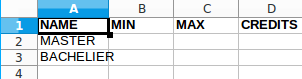
\includegraphics[width=\textwidth]{excel_programs_ex}
\end{figure}

\begin{figure}
\centering
\caption{La page relative aux cours d'un template de formulaire}
\label{fig:excel_courses_ex}
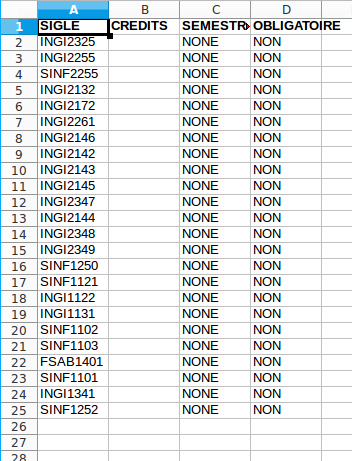
\includegraphics[width=\textwidth]{excel_courses_ex}
\end{figure}

\begin{figure}
\centering
\caption{La page relative aux modules d'un template de formulaire}
\label{fig:excel_modules_ex}
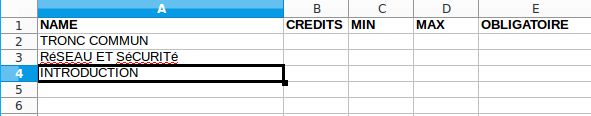
\includegraphics[width=\textwidth]{excel_modules_ex}
\end{figure}

\begin{figure}
\centering
\caption{Un catalogue de cours après sa création}
\label{catalog_show}
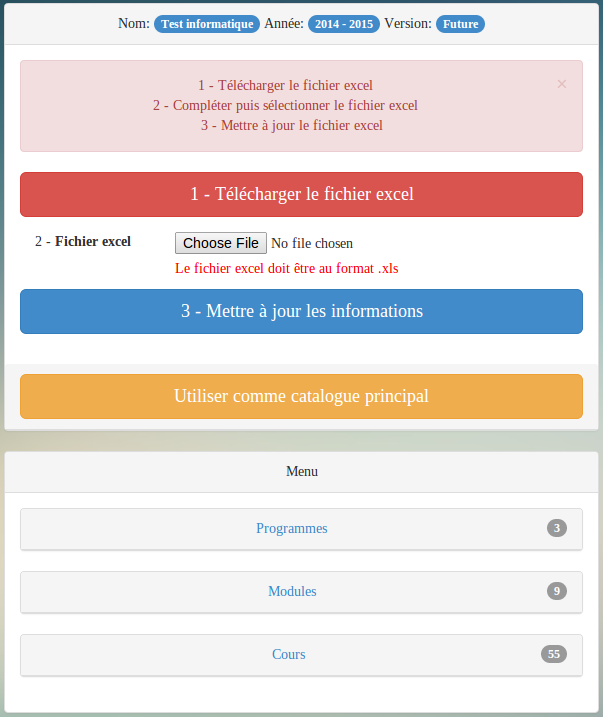
\includegraphics[width=\textwidth]{catalog_show}
\end{figure}

Toute ces fonctionnalités sont accessible depuis la page telle qu'elle est illustré sur l'image \ref{fig:catalog_show}. Via le menu à droite, les différents ensembles et cours du catalogue sont accessible. En haut à gauche apparaissent les trois propriétés identifiant notre catalogue, à savoir son nom, son année académique et sa version. 

En naviguant dans les différents sous menu du catalogue (cours, programmes, modules), vous pouvez accéder aux informations complètes concernant ces objets. Il est possible par exemple d'accéder aux détails des contraintes d'un cours. Il est notamment possible de créer des programmes de cours \textit{customisés} à partir des informations présentes dans le catalogue (cours, modules). On pourrait donc par exemple créer un programme \textit{Erasmus} ou \textit{Mercator} avec les modules et cours disponibles, pour proposer aux étudiants étrangers un programme de cours adapté à leur profil.

\subsubsection{Gérer les années des étudiants}
Bien qu'elle ne soit pas mentionné sur le diagramme \ref{fig:desired_process}, la fonctionnalité qui permet à la commission de programme de marquer les années des étudiants comme réussie, ou comme ratée (en sélectionnant les cours réussis) est relativement importante pour le bon fonctionnement du module qui s'occupe de vérifier les contraintes. 


En effet, pour vérifier la valider des contraintes de type \textit{dépendance} (se référer à  la section \ref{dependances} pour plus de détails), il est nécessaire de différencier les années réussies des années ratées, et de différencier, dans ces années ratées, les cours réussis des cours ratés. Ainsi, le module qui vérifie les contraintes ne prendra pas en compte un cours qui est présent dans une année mais qui n'a pas été réussi lorsqu'il vérifiera certaines dépendances. 

Pour les mêmes raisons, il est primordial de garder une trace des années ratées de l'étudiant, pour savoir quels cours l'étudiant a validé durant cette année qu'il n'a pas réussi.

On peut donc gérer sur la page \ref{fig:year_mgmt} les années des étudiants. Marquer une année comme réussie ou ratée empêchera à l'avenir l'étudiant de modifier ou de supprimer son année dans la page de gestion de son programme. Pour marquer son année comme ratée, il suffit de sélectionner les cours qu'il a réussi (comme on peut le voir sur la figure \ref{fig:failed_year_mgmt})
\begin{figure}
\centering
\caption{La page de gestion des années}
\label{fig:year_mgmt}
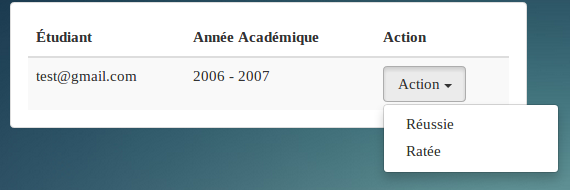
\includegraphics[width=\textwidth]{year_mgmt}
\end{figure}

\begin{figure}
\centering
\caption{Gérer une année ratée}
\label{fig:failed_year_mgmt}
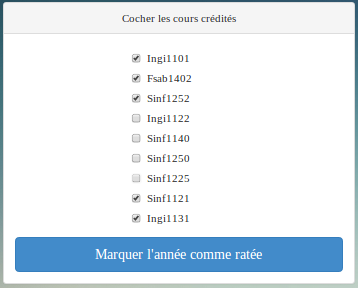
\includegraphics[width=\textwidth]{failed_year_mgmt}
\end{figure}


\subsubsection{Gérer les demandes de validations}
\subsection{Fonctionnalité de l'application - Étudiant}

Cette fonctionnalité s'occupe de gérer les étapes \textit{Négociation avec l'étudiant et Valider le programme de l'étudiant} du processus représentée sur le diagramme \ref{fig:desired_process}. 

Lorsqu'un étudiant pense que son programme est correct, il envoie une demande de validation à la commission de programme. Dans le meilleur des mondes, le programme de l'étudiant respecte toute les contraintes imposées par le programme qu'il suit. Cependant, pour une raison X ou Y, il arrive qu'un étudiant pense avoir une bonne raison pour enfreindre une ou plusieurs contraintes.

Prenons l'exemple d'un étudiant en provenance d'une autre université qui vient suivre un programme de master à l'UCL. En regardant attentivement l'exemple fictif \ref{fig:running_example}, on s’aperçoit que le cours \textit{INGI2315} du programme de master a une dépendance (\textit{SINF1140}) dans le programme de bachelier. Lorsque l'étudiant construit son programme de MASTER, il va se trouver avec des contraintes non respectées qu'il ne sera pas possible pour lui de corriger. 

Comme expliquer dans la section relatives au fonctionnalités offertes à l'étudiant qui suit \ref{validation_request}, l'application permet à l'étudiant, sous certaines conditions (remplir une justification s'il subsiste des contraintes non vérifiées par exemple), de soumettre un programme non valide à la validation. Lorsque notre étudiant soumettra son programme, il remplira un formulaire de justification avant d'envoyer sa demande de validation.

La page qui donne accès à la commission de programme aux demandes de validations est la suivante \ref{fig:validation_mgmt}. Sur cette page, la commission de programme peut accéder aux programmes de l'étudiant (Menu Programme), accéder aux contraintes non-vérifiées du programme (Menu Exceptions) et se rendre sur l'outil de messagerie (Menu Justifications). L'outil de messagerie est relativement simple et permet (seulement) aux deux parties de s'échanger des messages, sur base de la justification initiale de l'étudiant (Figure \ref{fig:messenger})



\begin{figure}
\centering
\caption{Page de gestion des demandes de validation}
\label{fig:validation_mgmt}
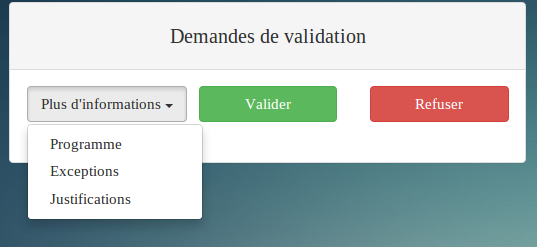
\includegraphics[width=\textwidth]{validation_mgmt}
\end{figure}

\begin{figure}
\centering
\caption{Communication entre la commission et un étudiant}
\label{fig:messenger}
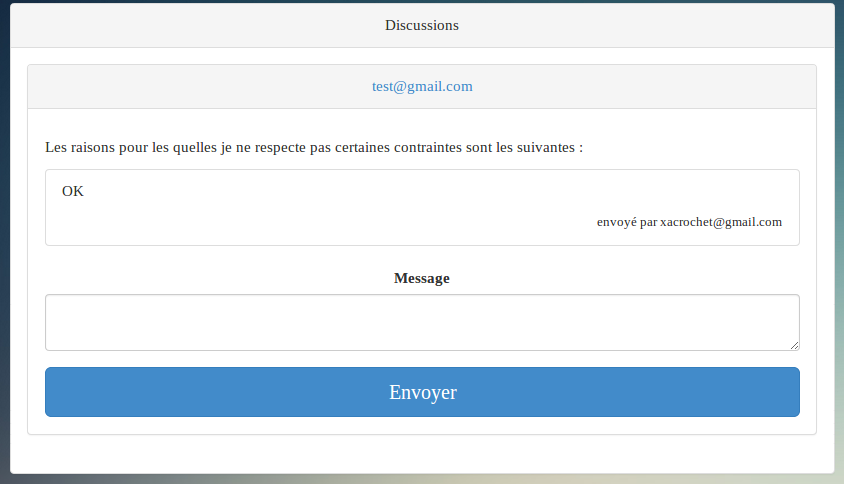
\includegraphics[width=\textwidth]{messagerie}
\end{figure}



% BOUGER VERS DEV
% \subsection{Contraintes}

% \subsection{Gestion des Données}
% \label{gestion_des_données}
% \subsubsection{Introduction}
% Cette section répond à la question de comment sont importées les données relatives aux programmes, leur cours, leurs informations et leur différentes contraintes. 

% Les différentes informations contenue dans le catalogue de cours du département sont les suivantes. Nous avons
% \begin{itemize}
% \item Plusieurs programmes de cours (BAC SINF et INFO, MASTER SINF et INFO, Passerelle SINF et toute les options qu'elles contiennent)
% \item Chacun de ces programmes contiennent des modules et des cours, avec des informations relatives aux cours et modules obligatoires.
% \item Chacun de ces cours peut avoir des dépendances. (Voir section contrainte pour plus de détails)
% \end{itemize}

% Il faut donc trouver un moyen de télécharger ces informations dans l'application. La solution la plus naïve serait de fournir des formulaires pour chaque entité (Cours, modules, ...) permettant d'ajouter une à une toute les informations nécessaire. Si l'on veut modifier les informations d'une entité, \textit{"il suffirait"} de naviguer dans les différents menu et de sélectionner le menu d'édition correspondant. Cependant cette solution n'atteint pas l'objectif fixé dans la solution, à savoir fournir un support pour enregistrer efficacement (et donc en peu de temps) les informations relatives aux curricula. Ajouter une à une toute les dépendances de cours peut être très ennuyant. 

% Une première amélioration que l'on peut ajouter à cette solution, est d'utiliser des formulaires excel pour ajouter ces informations. En créant une page par entité comme présenté sur l'image~\ref{fig:excel_example}, on pourrait ajouter toute les informations liés au modules, aux cours plus efficacement, l'import de fichier excel étant une chose assez aisée. 
% \begin{figure}[H]
% \centering
% \caption{Feuille Excel pour importer les données relatives aux modules}
% \label{fig:excel_example}
% 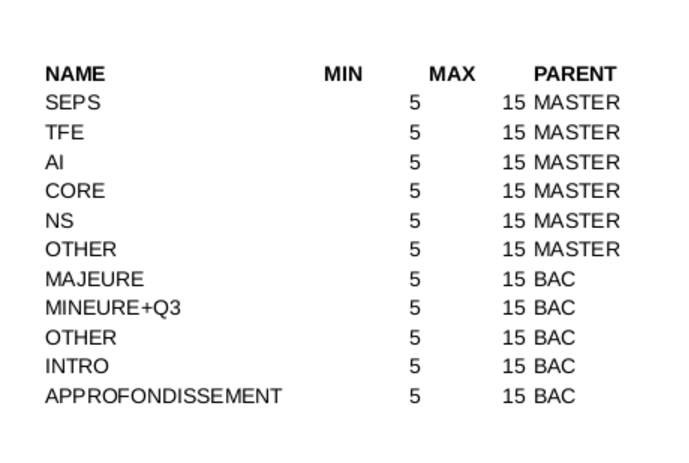
\includegraphics[width=0.8\textwidth]{excel_example}
% \end{figure} 

% Bien que cela permette d'ajouter des informations de façon plus efficaces, il subsiste plusieurs problèmes
% \begin{itemize}
% \item C'est toujours aussi éprouvant d'ajouter les dépendances. Il toujours les ajouter une par une, bien que cela soit sur une seule page.
% \item On ne peut pas donner au formulaire (et le programme qui l'importe) le pouvoir de créer les entités car:
% \begin{itemize}
%   \item En cas de faute de frappe, il faudra de nouveau naviguer dans l'application pour supprimer les erreurs.
%   \item Il est très difficile et peu efficace de gérer les inclusions des cours(L'appartenance d'une entité à une autre, un cours à un module par example). Cela implique des recherches sur le nom des entités. De nouveau, en cas de faute de frappe, il faudra aller corriger les erreurs dans l'application
% \end{itemize}
% \end{itemize}

% Le catalogue de cours étant un graphe (Dont les nœuds sont des entités et les dépendances des arrêtes), une autre solution serait d'utiliser un logiciel qui permet d'en dessiner. Un graphe étant visuellement plus parlant  qu'un tableur, le nombre d'erreurs serait donc moindre. 

% Le principal problème de cette solution réside dans les informations que l'on peut mettre dans ce graphe. Certes, on pourrait \textit{bricoler} avec le logiciel pour ajouter des méta-données aux objets que l'on dessine, mais cela pourrait de nouveaux devenir très embêtant à utiliser et surtout relativement compliqué à importer. 
  
% La solution utilisée dans l'application est un compromis entre la solution \textit{"graphe"} et celle \textit{"excel"}. La gestion des données est subdivisées en deux processus:
% \begin{itemize}
% \item L'import de la structure du catalogue via un logiciel qui permet de dessiner des graphes
% \item L'ajout d'informations supplémentaires (Nom, crédits, ...) via un import de formulaire excel
% \end{itemize}
% \subsubsection{Pourquoi avoir subdiviser l'import des données en deux parties distinctes?}

% Pour rendre les choses plus aisées au personnel qui va encoder le programme, nous avons décidé d'utiliser yEd, un outil relativement haut niveau qui permet de générer des graphes. En peu de temps, il est possible de construire l'ensemble du programme de cours à l'aide de cet éditeur disponible sur Windows, Mac Os et Linux tout en sortant un diagramme clair et concis.


% \textbf{Pourquoi}? Car le programme de cours est un graphe, dont chaque nœud correspond à un cours et chaque \textit{edge}, à une dépendance. 

% La solution idéale serait d'avoir un logiciel qui, en plus d'être intégré à l'application serait totalement adapté à notre besoin, à savoir \textbf{dessiner un graphe de cours}. Cela serait un dessinateur de programme de cours à part entière, proposant des nœuds intitulés cours, des arrêtes pour exprimer les contraintes, une façon de regrouper ces nœuds en module, en plus d'une autre pour y ajouter des informations relatives aux crédits, au contraintes des modules, etc. Cependant, cela dépasse malheureusement le cadre de mon mémoire. Libre à un étudiant, féru de développement web, de s'y attaquer dans les années à venir.

% \subsubsection{Limites de la démarche}
% Pour revenir à la façon dont nous importons les données, la principale limite d'un outil de la sorte est que nous sommes limités dans l'information que nous pouvons mettre dans ce graphe. Certes, il serait possible de sélectionner les différents nœuds et modules un à un et d'y ajouter l'information nécessaire, mais cette solution n'est pas efficace. Ils existe des solutions plus efficaces pour gérer des données à grande échelle : Excel.

% La seconde limite, est qu'il faut se mettre d'accord sur l'utilisation de ce programme tiers afin de savoir \textit{quoi} parser. Tout cela sera détaillé dans un manuel disponible dans les annexes

% L'import des données se fait donc en deux temps. Le graphe, qui contient les informations sur la structure du catalogue de cours (Nom des différentes entités et des dépendances), est d'abord parsé par l'application pour en extraire les informations. En suite, les informations plus spécifiques du catalogue de cours (les propriétés diverses des entités; nom détaillé, url, date, informations sur les crédits) doivent être fournies via un formulaire Excel qui, à sont, tour doit être télécharger vers l'application.

% \subsubsection{Construction et Import de la structure du catalogue}
% L'idée est de construire le graphe de cours en utilisant une application externe. Les exigences pour ce logiciel sont les suivantes:
% \begin{itemize}
% \item  Avec ce logiciel, il doit être possible de grouper les différents nœuds pour représenter les curricula et leur différents modules.
% \item Le graphe étant relativement complexe, il est nécessaire d'avoir un outil qui arrive à construire une disposition correcte
% \item Il doit être possible d'exporter ces informations dans un format standard et aisé à parser. 
% \item Ce logiciel doit être disponible sur Mac Os, Linux et Windows. 
% \end{itemize}

% Plusieurs candidats on été retenus; yEd, Dia et Graphiz. Tout les trois sont disponibles aussi bien sur Windows et Mac os que sur Linux et permettent d'exporter dans un format standard : le xml, mais un seul d'entre-eux permet de restructurer dynamiquement la structure du graphe: yEd.

% C'est pourquoi notre choix c'est porté sur ce logiciel.

% L'idée, pour construire le catalogue de cours, est (Dans yEd)
% \begin{itemize}
% \item D'utiliser les nœuds pour ajouter des cours, et de les labelliser avec leur sigle.
% \item D'utiliser les différents types d'arêtes pour représenter les différents types de dépendances
% \item De mettre les nœuds dans des groupes (labellisés avec leur nom) et les groupes dans des autres groupes pour représenter les différents modules, sous modules et programmes
% \end{itemize}

% Après, on demande au programme de calculer un layout hiérarchique. Sur l'image suivante, vous pouvez voir une partie de ce que génère yEd. (Le programme entier est disponibles dans les annexes)
% \begin{figure}[H]
% \centering
% 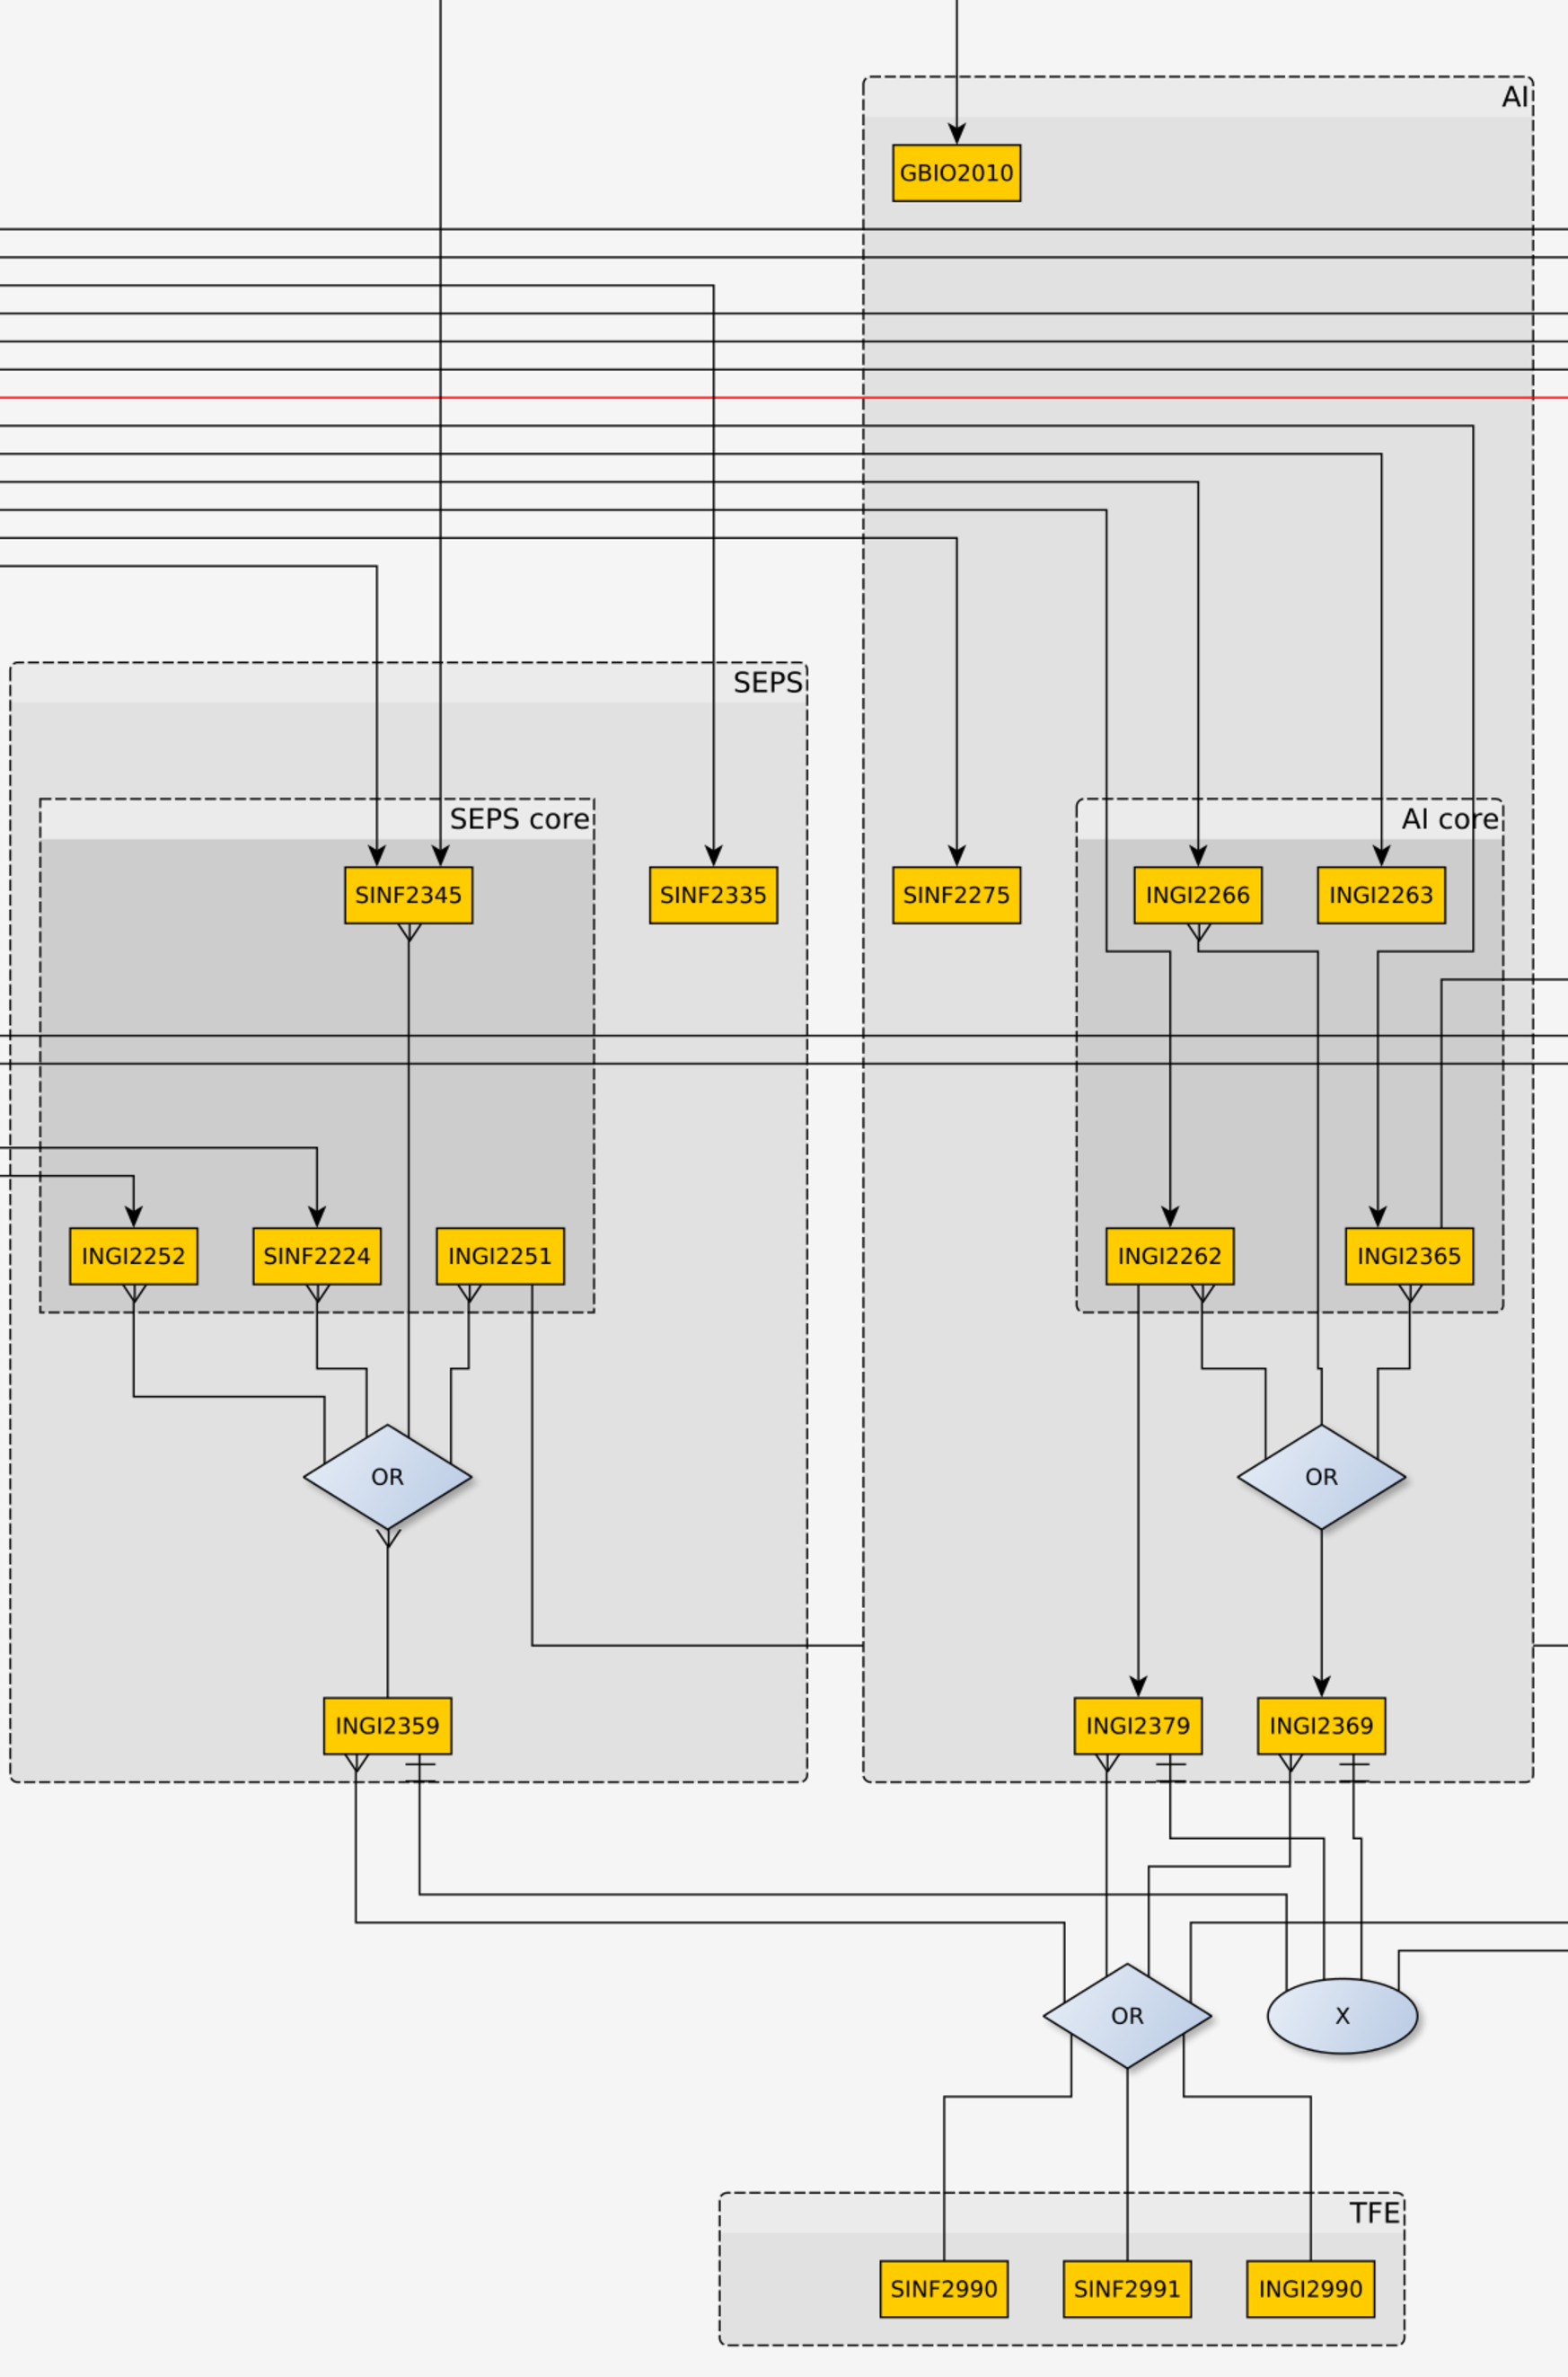
\includegraphics[width=\textwidth]{ingi_sub_course_catalog}
% \caption{Exemple de graph généré par Yed}
% \label{fig:subcatalog}
% \end{figure}


% \subsubsection{Construction et Import du formulaire Excel}
% Comme expliqué précédemment, le graph à lui seul n'est pas suffisant pour ajouter toute les informations nécessaire à l'application. Le formulaire Excel est utilisé pour ajouter les informations relatives au propriétés des programmes, modules et cours des différents curricula. 

% Ces propriétés contiennent des informations simples sur les différents objets du catalogues comme le nom complet des différents cours, modules et programmes, les professeurs, les liens vers pages des cours. Elle contiennent aussi les informations relatives aux contraintes sur les propriétés, comme le nombre de crédits.

% Il n'y a aucune restrictions sur les informations qui peuvent être ajoutées ici. 

% La structure du document est la suivante~\ref{fig:excel_structure}. Tout d'abord, il y a une page par objet (Cours, Programme, Module, Sous-module)

% \begin{figure}[H]
% \centering
% \caption{Structure d'un formulaire Excel}
% \label{fig:excel_structure}
% 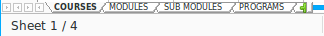
\includegraphics[width=0.8\textwidth]{excel_structure}
% \end{figure}

% Chacune des pages est structurée comme illustré sur l'image~\ref{fig:excel_page_structure}. 

% \begin{figure}[H]
% \centering
% \caption{Structure de la page relatives aux cours du formulaire Excel}
% \label{fig:excel_page_structure}
% 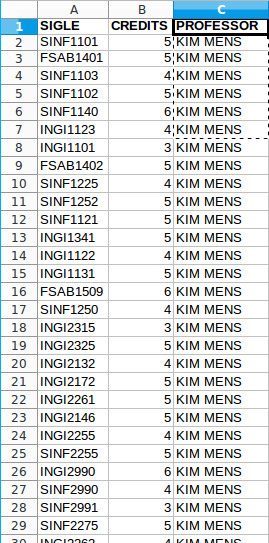
\includegraphics[scale=1]{excel_page_structure}
% \end{figure}

% La ligne 1, comprenant des cellules écrites en \textbf{gras} représente le header de la page. Chacune des cellules représente le nom de la propriété en question. Une propriété est un couple (Type, Value) où \textit{Type} correspond au nom de la propriété, et \textit{Value} à sa valeur. La première colomne représente la propriété qui \textbf{identifie} l'objet en question. Lorsque la page sera importé, une nouvelle propriété sera créée pour l'objet identifié par l'élément de la première colonne. La valeur de cette propriété sera la cellule traitée, et le type de la propriété le nom de la colonne. 

% Par exemple, pour la ligne 4 de la page~\ref{fig:excel_page_structure}
% Deux propriétés seront crées pour le cours intitulé \textit{SINF1103}
% \begin{enumerate}
% \item La propriété ayant pour type \textbf{CREDITS} avec comme valeur \textbf{5}.
% \item La propriété ayant pour type \textbf{PROFESSOR} avec comme valeur \textbf{KIM MENS}.
% \end{enumerate}

% Pour plus de facilité, il est possible de télécharger un \textit{template} de se formulaire depuis l'application, contenant toute les informations qui existe dans la base de données. 

% Par example, si l'on décide de télécharger ce template juste après avoir importer le graphe de cours, on aura les informations suivantes~\ref{fig:init_excel} pour les cours. 

% \begin{figure}[H]
% \caption{Formulaire excel téléchargé juste après importation du graphe}
% \label{fig:init_excel}
% 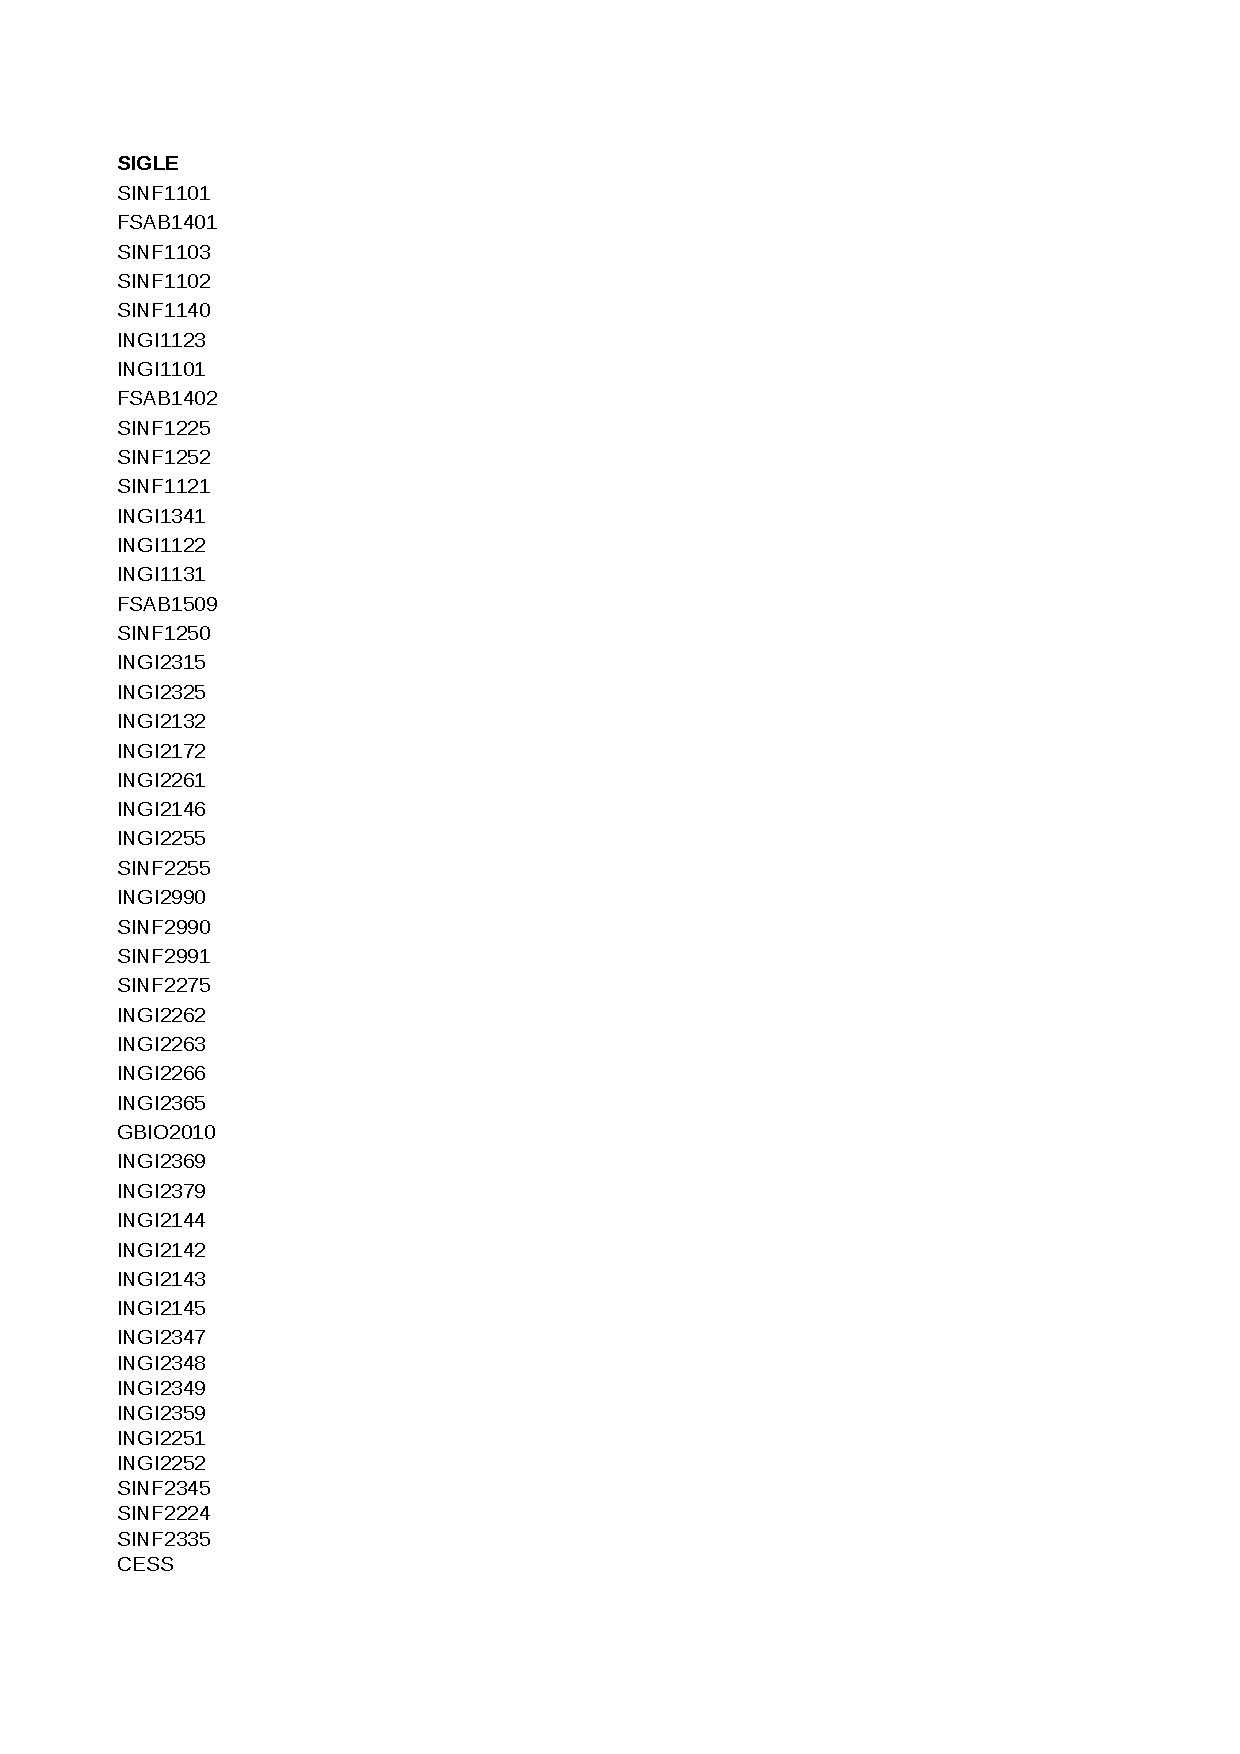
\includegraphics[scale=0.8]{init_excel}
% \end{figure}

% Il suffira après à la commission de programme de compléter ce fichier avec les informations souhaitées et de le télécharger vers l'application.

%         